\chapter{Lecture 11 Sparse Matrices and Iterative Solution Methods}
\label{ch:lec11n}
\section{Objectives}
The objectives of this lecture are to:
\begin{itemize}
\item Describe sparse matrices and their importance in scientific computing.
\item Introduce iterative solution methods.
\item Show some examples.
\end{itemize}
\setcounter{lstannotation}{0}

\section{Introduction}
Up to this point we have discussed a handful of methods for solving linear systems of equations.  We studied Gauss elimination with and without pivoting; LU factorization which, to be sure, is basically the same as Gauss elimination.  We also learned a little bit about the array of solution methods that are used in MATLAB's built-in tools for linear equations such as the QR factorization and LDL and Cholesky factorizations.  These are fundamental methods that should be in the toolbox of every engineer.

There are practical situations where these direct solution methods for linear equations are not suitable.  Physical conservation laws that are encoded in partial differential equations, discretized and solved using methods like the finite element method (FEM) and finite volume method (FVM) result in large systems of linear equations.  A high-resolution simulation will routinely require upwards of $10^5$ degrees of freedom\sidenote{In this context, the number of \emph{degrees of freedom} can be interpreted to refer to the length of a vector describing the unknown function.} to adequately resolve the physics of interest such as: the flow field around an automobile to estimate drag forces; stress and strain distribution within a complex structural component to ensure material failure limits are not exceeded; or the component temperature in the vicinity of a weld process.

Just \emph{storing} the matrices used to represent these linear systems---something, for example, like a $10^5 \times 10^5$ matrix\sidenote[][-1.25cm]{Such a matrix has $10^{10}$ entries.  If each entry is represented with a double-precision floating point number (8 bytes each), that adds up to roughly 80 Gigabytes of memory just to \emph{store} the matrix.}---requires us to take a new approach from what we have described up to now.  Likewise solving the systems to find the unknown vectors---whether the vector represents temperature, pressure, a velocity component, or a component of material displacement---requires new techniques.

\section{Sparse Matrices}

Matrices that arise as part of a finite difference method or finite element method are almost always \emph{sparse}.  This means that for every row of the matrix, corresponding to a linear equation pertaining to a single degree of freedom, most of the entries are equal to zero.  

\begin{marginfigure}[-3.75cm]
%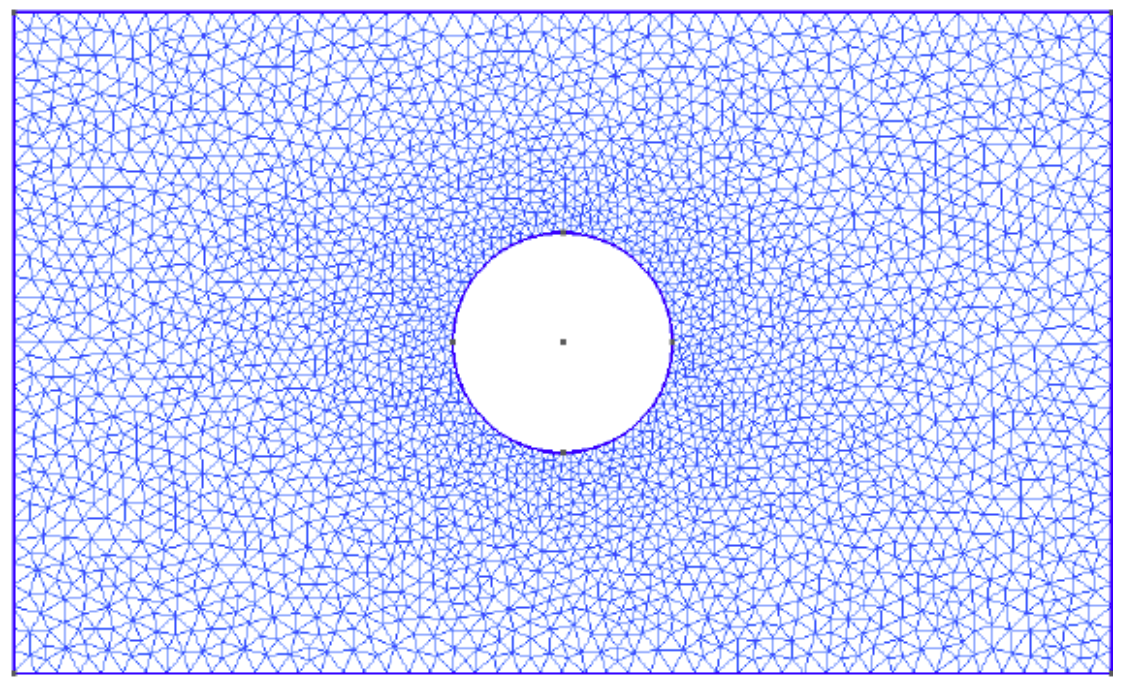
\includegraphics{lec11n-mesh.png}
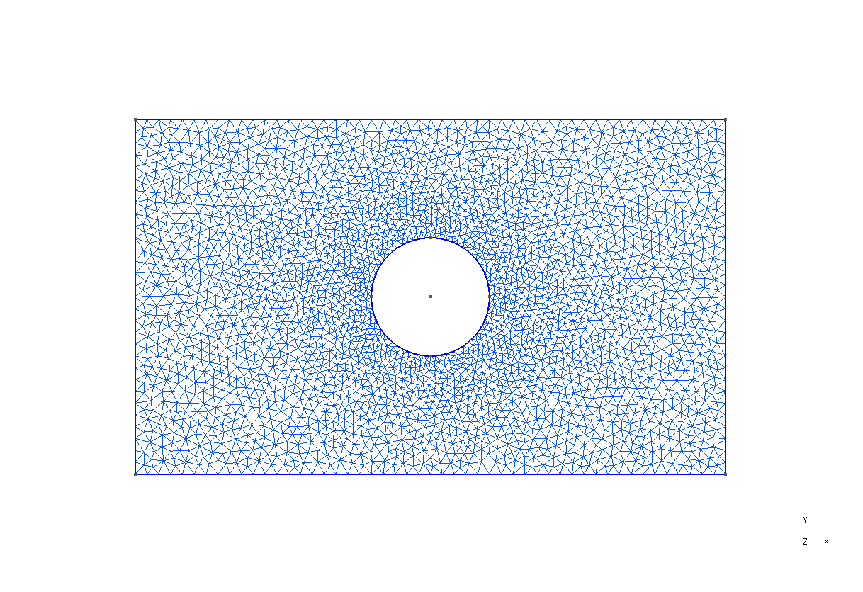
\includegraphics{discretization.eps}
\caption{A triangular mesh for a finite element method analysis of the transient heat equation.}
\label{fig:lec11n-mesh}
\end{marginfigure}
As an example, consider a finite element discretization of the transient heat equation on a domain that is rectangular in shape, but with a hole in the middle.  The mesh is depicted in Figure \ref{fig:lec11n-mesh}. The governing equation is shown in Equation \ref{eq:lec11n-transient-heat}:
\begin{equation}
\frac{k}{\rho c_p}\frac{\partial u}{\partial t} = \nabla^2 u + S
\label{eq:lec11n-transient-heat}
\end{equation}
where $k$ is the thermal conductivity, $\rho$ is density, $c_p$ is the specific heat, $S$ corresponds to a constant uniform heat source, $u$ is the temperature, and $t$ is time. In the finite element method, this equation and specified boundary conditions are translated into a linear system of equations:
\begin{equation*}
Au = b
\end{equation*} 
\begin{marginfigure}[-6.0cm]
%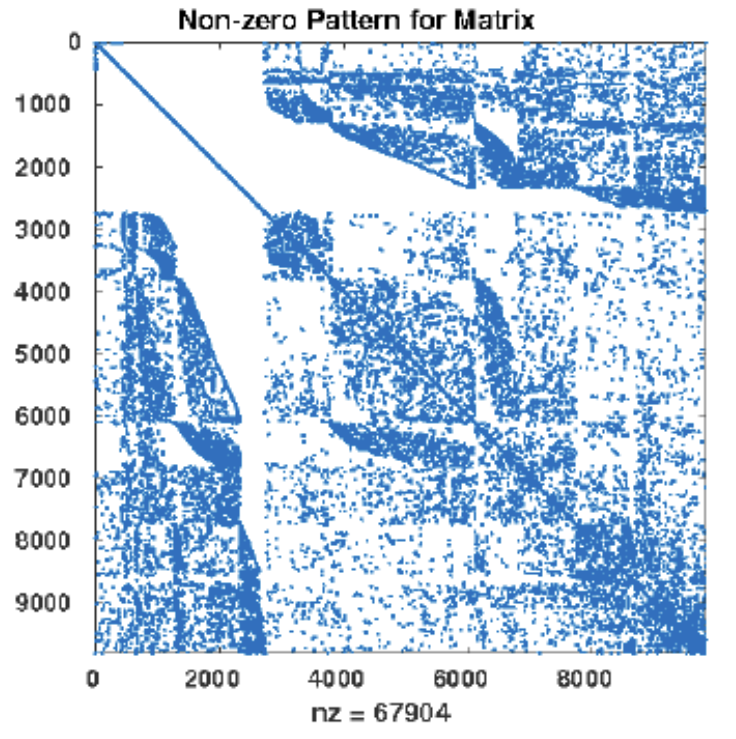
\includegraphics{lec11n-spy1.png}
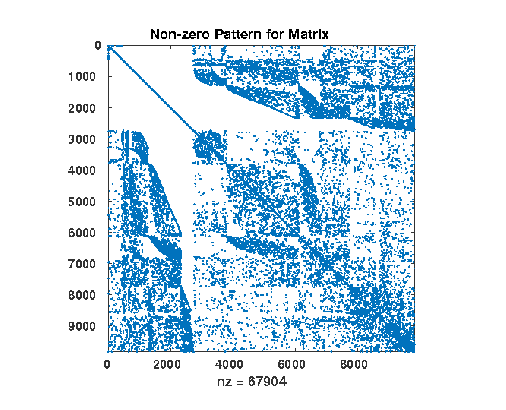
\includegraphics{Thermal_9824.eps}
\caption{Non-zeros in linear system for transient heat conduction.}
\label{fig:lec11n-spy1}
\end{marginfigure}
The non-zero structure of this system of equations can be observed using MATLAB's built-in function \lstinline[style=myMatlab]{spy(A)}, and the result is shown in Figure \ref{fig:lec11n-spy1}. The system of equations has 9824 nodes, each with a single degree of freedom.  The resulting $9824 \times 9824$ matrix $A$ has a total of 67,904 non-zero entries; an average of about 8 non-zero elements per equation.\sidenote[][-3.0cm]{Bottom Line Up Front: this number of non-zeros per row is typical for two-dimensional systems with linear, triangular elements.  The number of non-zeros per equation for the FEM or FVM depends on a number of factors: a) number of degrees of freedom per node; b) the number of spatial dimensions; c) the number of internal degrees of freedom for each finite element, among other factors.  This will be discussed in detail in later lectures on finite element methods.  } This pattern, which is typical for such matrices, can be exploited by only storing and carrying out arithmetic with the non-zero entries of the matrix.  

There are a number of sparse-matrix storage formats in use.  MATLAB uses the compressed-sparse-column (CSC) storage format.\cite{gilbert1992sparse}  If there are $nnz$ non-zero entries in a $n \times n$ sparse array, MATLAB stores one (double precision) vector of length $nnz$ with the non-zero values---call this vector: \lstinline[style=myMatlab]{ENTRY}; another vector of integers of length $nnz$---call this vector: \lstinline[style=myMatlab]{ROW}---with the row-number for each non-zero; and a third vector of integers of length $n+1$---call this vector: \lstinline[style=myMatlab]{COL}---that stores the index (from the \lstinline[style=myMatlab]{ENTRY} array) of the first non-zero from each column and terminated with $nnz+1$.  An example of this format is shown in Figure \ref{fig:lec11n-csc}. \begin{marginfigure}
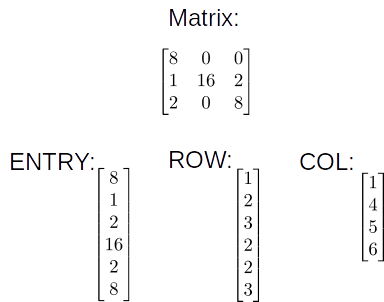
\includegraphics{CSC-example.png}
\caption{Example sparse matrix in Compressed Sparse Column format.}
\label{fig:lec11n-csc}
\end{marginfigure} The total storage required is $nnz \times 8$ bytes for the \lstinline[style=myMatlab]{ENTRY} array + $nnz \times 4$ bytes for the \lstinline[style=myMatlab]{ROW} array + $(n+1) \times 4$ bytes for the \lstinline[style=myMatlab]{COL} array.  In asymptotic notation, $\mathcal{O}(nnz+n)$ bytes of storage are required.  Contrast this with $\mathcal{O}(n^2)$ for dense matrices.  If $nnz << n$ the savings with sparse matrices is huge.  The key issues to keep in mind are these:\marginnote{In terms of FLOPs, sparse matrix calculations are slower.  Dense matrix algorithms are heavily optimized to make best use of the memory hierarchy of common computer architectures resulting in high computational intensity---calculations performed for each byte loaded from memory---and consequently achieve high performance.  Sparse matrix algorithms have lower computational intensity and the memory access patterns are harder to optimize for multi-threaded execution.  As a result, sparse matrix operations are relatively slow.  Readers are encouraged to experiment with MATLAB to get a better feel for the relative performance of dense and sparse matrix operations.}
\begin{enumerate}
\item Exploiting the sparsity of these matrices is not a performance enhancement, it is a necessity.  Simulations of practical interest often result in systems of equations that can \emph{only} be stored as a sparse matrix.
\item The resulting matrix, if it is to be solved, \emph{cannot} be solved by Gauss elimination related algorithms like LU-factorization.
\end{enumerate}

The reason for the second point is that, even for matrices that are sparse, the LU-factorization (or modified coefficient array for Gauss elimination) for that matrix usually is not sparse.  The forward elimination process common to both of the aforementioned techniques systematically destroys the sparsity pattern.  This effect is shown in Figure \ref{fig:lec11n-LandU}.
\begin{figure}[h!]
\subfloat[]{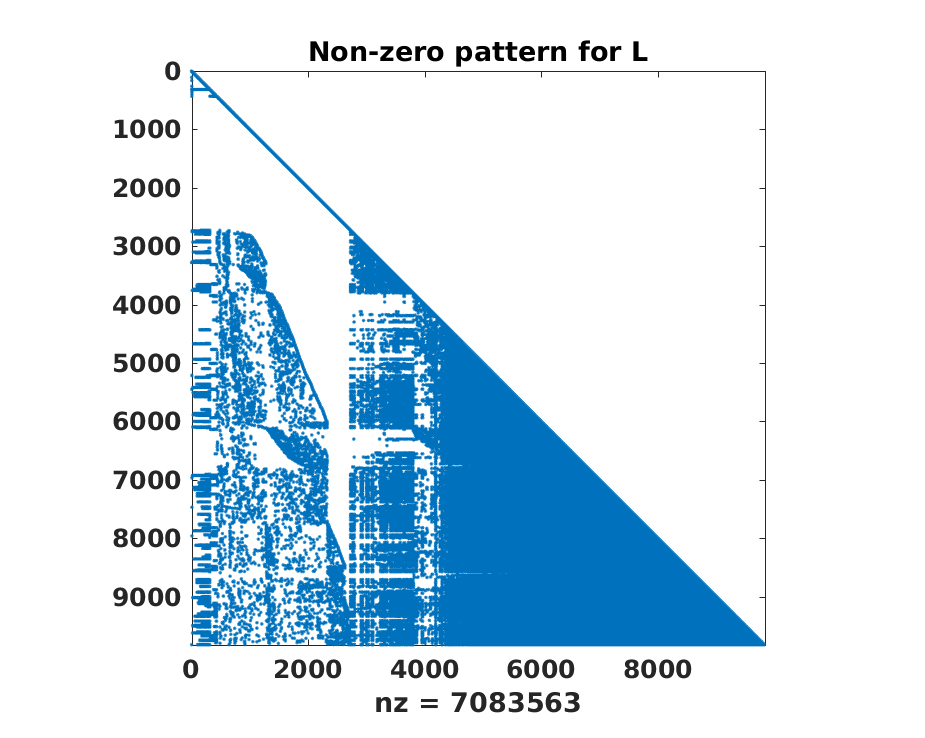
\includegraphics[width=2in]{Non_zero_L_thermal.eps}}
\subfloat[]{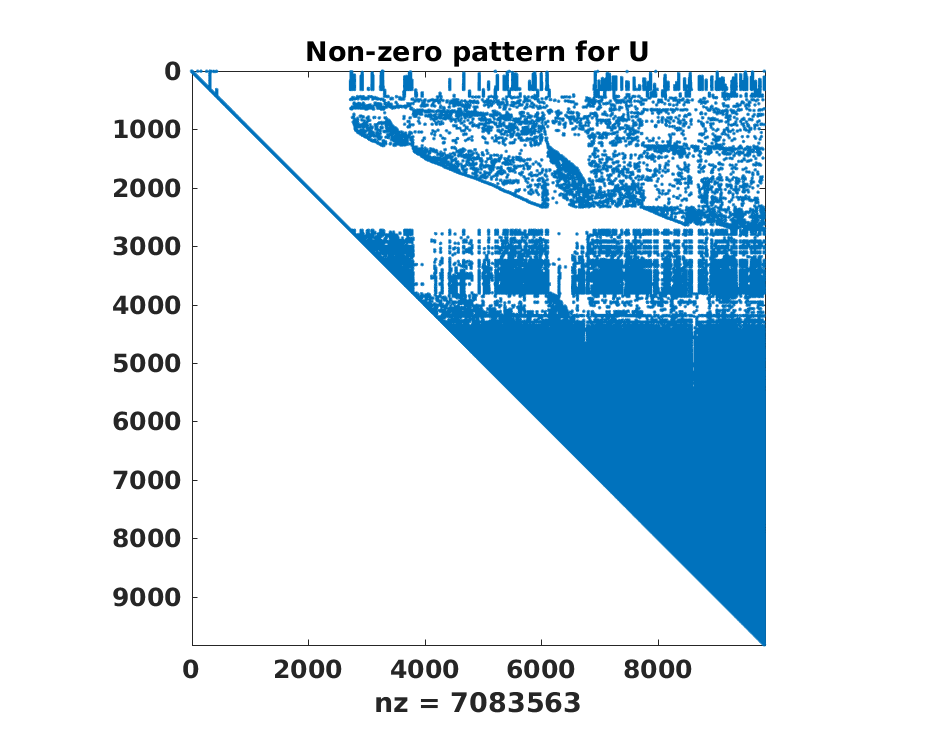
\includegraphics[width=2in]{Non_zero_U_thermal.eps}}
\label{fig:lec11n-LandU}
\caption[][3.0cm]{Sparsity pattern of L and U matrices from decomposition of A.}
\end{figure}

\noindent For the larger systems of equations that we want to solve for more interesting problems, this kind of fill-in defeats any benefit obtainable through use of sparse matrices.

\section{Iterative Solution Methods}

The fundamental idea of iterative methods for solving linear systems of equations is this: given an estimate of the solution, $x^{(k)}$, find a method to generate a new estimate, $x^{(k+1)}$, that is easy to compute and that ultimately converges to the solution of $Ax=b$.  Some of the methods that we will discuss in this lecture all involve \emph{splitting} the matrix $A$ into a decomposition $A=M-K$ with $M$ non-singular and very easy to invert.  If this is done, the iterative scheme is as follows:
\begin{align*}
Ax &= b \\
(M-K)x &= b \\
\rightarrow Mx &= Kx + b \\
\rightarrow x &= M^{-1}(Kx + b) \\
&= \underbrace{M^{-1}K}_{R}x + \underbrace{M^{-1}b}_{c}
\end{align*} \marginnote[-3.0cm]{\textbf{Note:} The matrix $R$ plays an important part in the mathematical theory of iterative methods. One relevent result is that if $$||R|| < 1$$ in some matrix norm, then the iterative method will converge. To the best of my knowledge, this is \emph{why} we carry out this business with splitting.}
The resulting iterative method is shown in Equation \ref{eq:lec11n-iterative-gen}:
\begin{equation}
x^{(k+1)} = Rx^{k} + c
\label{eq:lec11n-iterative-gen}
\end{equation}
where $k$ is the iteration number.

Instead of solving a system of equations by factoring the coefficient matrix, we create what we hope to be a convergent sequence of approximations to the solution by repeated matrix-vector multiplication.  Each matrix-vector multiplication operation takes, for dense matrices, $\mathcal{O}(n^2)$ operations.  Since the matrix $R$ is sparse and operations with zero entries of the matrix are eliminated, each matrix-vector multiplication takes only $\mathcal{O}(n)$ operations.

\subsection{Jacobi Iteration}

In this method, $M$ is defined to be the diagonal of $A$, and $K$ is the sum of the strictly lower and upper triangular portion of $A$.\cite{demmel1997applied}
\begin{align}
M &= \text{diag}(A) \\
K &= \tilde{L} + \tilde{U}
\end{align}
where $-\tilde{L}$ is the strictly lower triangular part of $A$ and $-\tilde{U}$ is the strictly upper triangular part of $A$ so that:
\begin{equation*}
A = M - (\tilde{L} + \tilde{U})
\end{equation*}
For a diagonal matrix, the inverse is just the same matrix with the diagonal elements inverted:
\begin{equation*}
M^{-1} = \left[
\begin{matrix}
\frac{1}{a_{11}} & &  \\
 & \ddots & \\
 & & \frac{1}{a_{nn}} 
 \end{matrix}
\right]
\end{equation*}
The iterative method is thus expressed:
\begin{align*}
x^{(k+1)} &= Rx^{(k)} + c \\
&=M^{-1}(\tilde{L} + \tilde{U})x^{(k)} + M^{-1}b \\
&=M^{-1}b - M^{-1}\tilde{L}x^{(k)} - M^{-1}\tilde{U}x^{(k)} \\
&=M^{-1}\left[b - \tilde{L}x^{(k)} - \tilde{U}x^{(k)}\right]
\end{align*}
We have manipulated the matrix equations to arrive at a more familiar form of the equation for Jacobi iteration, which is shown in Equation \ref{eq:lec11n-Jacobi}:
\begin{equation}
x_i^{(k+1)} = \frac{1}{a_{ii}}\left[b_{i} - \sum\limits_{j=1}^{i-1}a_{ij}x_{j}^{(k)} - \sum\limits_{j=i+1}^{n}a_{ij}x_j^{(k)} \right]
\label{eq:lec11n-Jacobi}
\end{equation}
where we express the solution for one element of $x^{(k+1)}$ at a time and the matrix-vector products are shown explicitly. A simple implementation of Equation \ref{eq:lec11n-Jacobi} in MATLAB is shown in the following listing where \lstinline[style=myMatlab]{x_in} refers to $x^{(k)}$ and \lstinline[style=myMatlab]{x_new} refers to $x^{(k+1)}$:
\begin{lstlisting}[style=myMatlab]
for i = 1:rows
    x_new(i) = (1/A(i,i))*(b(i) - ... /*!\annotation{lst:ann11n-1}!*/
        A(i,1:(i-1))*x_in(1:(i-1)) - ... /*!\annotation{lst:ann11n-2}!*/
        A(i,(i+1):n)*x_in((i+1):n)); /*!\annotation{lst:ann11n-3}!*/
end
\end{lstlisting}
\marginnote[-2.0cm]{
\vspace{0.1cm}

\noindent \ref{lst:ann11n-1} $x(i) = M^{-1}(b - \cdots$

\vspace{0.1cm}

\noindent \ref{lst:ann11n-2} $\cdots \tilde{L}x - \cdots$

\vspace{0.1cm}

\noindent \ref{lst:ann11n-3} $\cdots \tilde{U}x)$
}

The Jacobi method will converge to a solution provided that $A$ is \emph{diagonally dominant}.\sidenote{This is a sufficient condition for convergence but not a necessary condition.  The only guarantee is that if $A$ is diagonally dominant, it will converge.}  A matrix is diagonally dominant if the following relation is true:
\begin{equation*}
|a_{ii}| > \sum\limits_{j=1, j\ne i}^{n} |a_{ij}|
\end{equation*}

The main advantages of the Jacobi method are that:
\begin{enumerate}
\item it is easy to implement; and
\item it is easy to parallelize. In principle, the elements of $x^{(k+1)}$ can be updated in any order or all at the same time.
\end{enumerate}

In the listing above, we do not take advantage of the ability to parallelize the Jacobi iteration.  If we were to do this in MATLAB, we would need to structure the iteration so as to maximize Matrix-vector operations rather than element-wise operations so heavily used above.  An improved implementation is shown below:
\marginnote[-0.75cm]{
\noindent \ref{lst:ann11n-4} The MATLAB function \lstinline[style=myMatlab]{diag(A)} returns a vector with just the elements on the main diagonal of \lstinline[style=myMatlab]{A}.  The expression \lstinline[style=myMatlab]{diag(diag(A))} returns a square, diagonal matrix with only the elements on the main diagonal of \lstinline[style=myMatlab]{A}.  

\vspace{0.1cm}

\noindent \ref{lst:ann11n-5} This line provides a sparse matrix equivalent to $M^{-1}$.

\vspace{0.1cm}

\noindent Both \lstinline[style=myMatlab]{K} and \lstinline[style=myMatlab]{M_inv} are represented as sparse matrices.
}
\begin{lstlisting}[style=myMatlab]
K = -(A - diag(diag(A)));  /*!\annotation{lst:ann11n-4}!*/
M_inv = sparse(diag(1./diag(A))); /*!\annotation{lst:ann11n-5}!*/

/*! 
(Code to set-up and start iteration)
 !*/

    x_new = M_inv*(K*x_in + b);

\end{lstlisting}
The performance improvement from using the vectorized implementation will depend on $A$ but for large matrices, each iteration will run much faster.  A performance comparison is shown in Figure \ref{fig:jacobi-performance} for $900 \times 900$ matrix run on a typical workstation using MATLAB R2022a.  The vectorized version obtains the same answer but was more than 700 times faster.  An important take-away from this example is: \emph{how you write your MATLAB code can \textbf{greatly} impact performance.}
\begin{marginfigure}
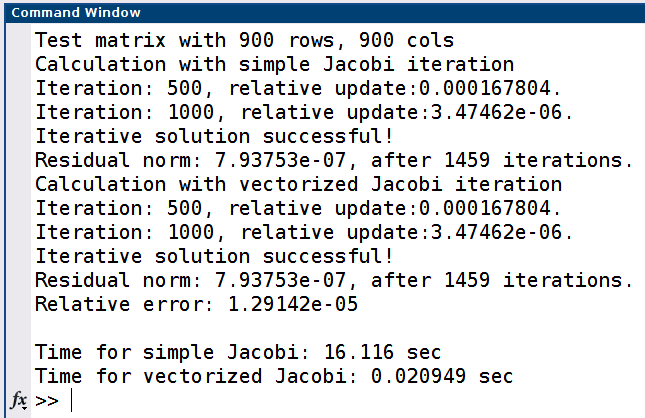
\includegraphics{jacobi-performance-comparison.png}
\caption{Jacobi method performance comparison for $900 \times 900$ test matrix.}
\label{fig:jacobi-performance}
\end{marginfigure}

The main disadvantage of the Jacobi method is \emph{slow convergence}; compared to other methods, it typically takes many iterations to achieve a solution within a specified error tolerance.

\section{MATLAB Implementation of Jacobi Method}
In this section we will present a full implementation of the Jacobi method.

As usual, we start by clearing out the workspace memory and command window output and close any figures.  We use a \lstinline[style=myMatlab]{switch...case} construct to allow selection between different linear systems.

\setcounter{lstannotation}{0}

\marginnote[2.5cm]{
\ref{lst:ann11n-1} A diagonally dominant test matrix.

\vspace{0.25cm}

\noindent \ref{lst:ann11n-2} We customarily use a zero vector for $x^{(0)}$.  In more complex schemes a simple alternative method is used to obtain a low-order approximation of the solution that can thus be used for $x^{(0)}$.  This, unsurprisingly results in faster convergence than the naive choice used here.

\vspace{0.25cm}

\noindent \ref{lst:ann11n-3} Here we use \lstinline[style=myMatlab]{show_x} as a flag to indicate whether or not we want to show the answer in the command window. If I set \lstinline[style=myMatlab]{show_x=1}, that indicates I want the solution, $x$, to be output to the MATLAB command window.  If \lstinline[style=myMatlab]{show_x=0} then $x$ is not output.  If $x$ is a vector with only a few elements, it is worthwhile to visually inspect the result and see that it is correct.  If $x$ has hundreds or thousands of elements, such exercises are useless.


\vspace{0.1cm}  

\noindent \ref{lst:ann11n-4} This is a $900 \times 900$ symmetric, positive definite matrix that has \emph{weak} diagonal dominance.  Weak diagonal dominance relaxes the requirement that the magnitude of the diagonal entry be greater than the sum of the absolute values of the off-diagonal entries; it can also be \emph{equal} to the sum of the off-diagonal elements.
}
\begin{lstlisting}[name=lec11n_jacobi, style=myMatlab]
%% Example: Jacobi Method Demonstration
clear
clc
close 'all'

sys_choice = 2;

switch sys_choice
    
    case 1
        A = [9 -2 3 2;
            2 8 -2 3;
            -3 2 11 -4;   /*!\annotation{lst:ann11n-1}!*/
            -2 3 2 10];
        b = [54.5;
            -14;
            12.5;
            -21];
        rows = 4; cols = 4;
        x_in = zeros(cols,1); /*!\annotation{lst:ann11n-2}!*/
        show_x = 1; /*!\annotation{lst:ann11n-3}!*/
           
    case 2
        [A,rows,cols,entries] = mmread('gr_30_30.mtx'); /*!\annotation{lst:ann11n-4}!*/
        fprintf('Test matrix with %d rows, %d cols \n',...
            rows,cols);
        b = rand(cols,1);
        x_in = zeros(rows,1);
        figure
        spy(A)
        title('Sparsity Pattern of Test Matrix')
        show_x = 0;

    otherwise
        error('Invalid system choice!\n');
end
\end{lstlisting}

We need to specify stopping criteria.  For iterative methods such as those under consideration in this lecture, one possible stopping criteria is shown in Equation \ref{eq:lec11n-iter-converge}.
\begin{equation}
\text{Estimated Relative Error} = \frac{|| x^{(k+1)} - x^{(k)}||_{\infty}}{||x^{(k)}||_{\infty}}
\label{eq:lec11n-iter-converge}
\end{equation}
This stopping criteria has the disadvantage that it does not provide any real assurance that $x^{(k+1)}$ is close to $x^{\star}$.  It only says that $x^{(k+1)}$ is close to $x^{(k)}$.  When evaluating the solution, you should also verify that the residual is small.\sidenote[][-2.0cm]{You might ask: why not just use the relative residual, $\sfrac{||Ax^{(k+1)} - b||}{||b||}$, as a stopping criteria?  My wan answer is: a lot of people use estimated relative error instead.  A somewhat better reason is that if the estimated relative error from Equation \ref{eq:lec11n-iter-converge} is very small, then $x^{(k)}$ is changing only slightly with more iterations and, if the answer is bad at that point, it probably will not get better any time soon.  My only advice is that you should check the relative residual when you are done to make sure your iteration did not converge to a garbage solution.}

The code listing below sets stopping criteria, invokes the Jacobi solver, and evaluates performance.
\marginnote[0.0cm]{

\noindent \ref{lst:ann11n-5} The MATLAB functions \lstinline[style=myMatlab]{tic} and \lstinline[style=myMatlab]{toc} act as a simple timing tool.  The call to \lstinline[style=myMatlab]{tic} starts the clock; when we call \lstinline[style=myMatlab]{toc} the clock is stopped and the elapsed time (in seconds) is returned and, in this case, assigned to the variable \lstinline[style=myMatlab]{time_jac}.

\vspace{0.1cm}

\noindent \ref{lst:ann11n-6} Here we make use of the \lstinline[style=myMatlab]{exit_code} returned from our function.  If \lstinline[style=myMatlab]{exit_code=1}, that means the iterative solver stopped based on the estimated relative error.  

\vspace{1.0cm}

\noindent \ref{lst:ann11n-7} Here we make use of the \lstinline[style=myMatlab]{show_x} variable.  In this context, if \lstinline[style=myMatlab]{show_x} is \emph{not} equal to zero, the Boolean expression \lstinline[style=myMatlab]{if show_x} evaluates as true and the \lstinline[style=myMatlab]{if...end} block is executed; in this case, displaying \lstinline[style=myMatlab]{x} to the MATLAB command window.

}
\begin{lstlisting}[style=myMatlab, name=lec11n_jacobi]
%% Solve using Jacobi Iteration

% set stopping criteria
imax = 1500; % max iterations
tol = 1e-7; % estimated relative error tolerance

fprintf('Calculation with simple Jacobi iteration \n');
tic;
[x_jac,norm_res,num_iter,exit_code] = ...  /*!\annotation{lst:ann11n-5}!*/
    jacobi_solver(A,b,x_in,tol,imax);
time_jac = toc;

if exit_code == 1  /*!\annotation{lst:ann11n-6}!*/
    fprintf('Iterative solution converged!\n');
    fprintf('Residual norm: %g, after %d iterations.\n',...
        norm_res,num_iter);
end

if show_x
   fprintf('x = \n'); disp(x_jac);  /*!\annotation{lst:ann11n-7}!*/
end

fprintf('Calculation with vectorized Jacobi iteration \n');
tic;
[x_jac_v,norm_res_v,num_iter_v,exit_code_v] = ...
    jacobi_solver_v(A,b,x_in,tol,imax);
time_jacv = toc;

if exit_code_v == 1
    fprintf('Iterative solution converged!\n');
    fprintf('Residual norm: %g, after %d iterations.\n',...
        norm_res_v,num_iter_v);
end

if show_x
   fprintf('x = \n'); disp(x_jac_v); 
end

\end{lstlisting}
As previously discussed, even if the iterative scheme converges, we should check the relative residual to see if we have converged to something like the correct solution.  Code to do this is in the next listing.
\marginnote[1.0cm]{
\ref{lst:ann11n-8} The relative residual calculation is implemented as part of the iterative schemes.  It is not used as a stopping criterion but is passed back as a return argument.
}
\begin{lstlisting}[style=myMatlab, name=lec11n_jacobi]
%% Check Relative Residual

fprintf('Relative residual Jacobi: %g \n',norm_res); /*!\annotation{lst:ann11n-8}!*/
fprintf('Relative residual vectorized Jacobi: %g \n',...
    norm_res_v);
\end{lstlisting}

Finally we present the full implementation of the Jacobi iteration.  The basic version is in the listing below:
\begin{lstlisting}[style=myMatlab, name=lec11n-jacobi]
%% Local functions
function [x_new,norm_res,num_iter,exit_code] = ...
    jacobi_solver(A,b,x_in,tol,imax)
[n,~] = size(A);
rel_update = inf;
x_new = x_in; % initialize x_new
for iter = 1:imax
    if (iter > 1) && (mod(iter,500) == 0)
        fprintf('Iteration: %d, relative update:%g. \n',...
            iter,rel_update);
    end 
    for i = 1:n
        x_new(i) = (1/A(i,i))*(b(i) - ...
            A(i,1:(i-1))*x_in(1:(i-1)) - ...
            A(i,(i+1):n)*x_in((i+1):n));
    end
    if norm(x_in,"inf") ~= 0 % prevent nan
        rel_update = ...
            norm(x_new - x_in,"inf")/norm(x_in,"inf");
    end    
    % check exit criteria
    if rel_update < tol
        exit_code = 1; % success
        break; % "break out" of the for loop
    end    
    if iter == imax
        % maximum iterations reached
        exit_code = 0; 
    end
    x_in = x_new;    
end
norm_res = norm(A*x_new - b,2)/norm(x_new,2);
num_iter = iter;
end
\end{lstlisting}
And the, slightly different, vectorized version:

\begin{lstlisting}[style=myMatlab, name=lec11n-jacobi]
function [x_new,norm_res,num_iter,exit_code] = ...
    jacobi_solver_v(A,b,x_in,tol,imax)
rel_update = inf;
x_new = x_in; % initialize x_new
K = -(A - diag(diag(A)));
M_inv = sparse(diag(1./diag(A)));

for iter = 1:imax
    if (iter > 1) && (mod(iter,500) == 0)
        fprintf('Iteration: %d, relative update:%g. \n',...
            iter,rel_update);
    end
    
    x_new = M_inv*(K*x_in + b);

    if norm(x_in,"inf") ~= 0 % prevent nan
        rel_update = ...
            norm(x_new - x_in,"inf")/norm(x_in,"inf");
    end    
    % check exit criteria
    if rel_update < tol
        exit_code = 1; % success
        break; % "break out" of the for loop
    end    
    if iter == imax
        % maximum iterations reached
        exit_code = 0; 
    end
    x_in = x_new;
    
end
norm_res = norm(A*x_new - b,2)/norm(x_new,2);
num_iter = iter;
end
\end{lstlisting}

\subsection{Gauss-Seidel Method}
The Gauss-Seidel method is a minor modification of the Jacobi method.  Recall the basic update scheme for the Jacobi iteration:
\begin{equation*}
x_i^{(k+1)} = \frac{1}{a_{ii}}\left[b_{i} - \sum\limits_{j=1}^{i-1}a_{ij}x_{j}^{(k)} - \sum\limits_{j=i+1}^{n}a_{ij}x_j^{(k)} \right]
%\label{eq:lec11n-Jacobi}
\end{equation*}
and notice that, when we are computing the update for $x_i^{(k+1)}$, if we are indeed carrying out these calculations sequentially for increasing values of $i$, we already have updated values of $x^{(k+1)}_j$ on-hand for $1 \le j < i$.  Why not use them?  Answer: there is no reason why not; let us use them.  The update scheme for Gauss Seidel is given in Equation \ref{eq:lec11n-GS}.
\begin{equation}
x_i^{(k+1)} = \frac{1}{a_{ii}}\left[b_{i} - \sum\limits_{j=1}^{i-1}a_{ij}x_{j}^{(k+1)} - \sum\limits_{j=i+1}^{n}a_{ij}x_j^{(k)} \right]
\label{eq:lec11n-GS}
\end{equation}
The good news is that use of updated values in this way results in the Gauss-Seidel method converging in roughly half as many iterations as the Jacobi method.  The bad news is that the order in which we calculate $x_{i}^{(k+1)}$ matters; we cannot do them in parallel like we could with the Jacobi method.\sidenote{And, perhaps it does not need to be mentioned, given that the vectorized Jacobi method is hundreds of times faster than the non-vectorized version, one may be hard-pressed to give up such an advantage.}  Still, the performance improvement from the vectorized implementation of Jacobi was \emph{heavily} dependent on the fact that we are working in a MATLAB environment.  It would be quite difficult to replicate an equivalent implementation if you were using, for example, C++ or FORTRAN.  So, if you \emph{could not} make use of the inherent parallelism of the Jacobi method, Gauss-Seidel would offer you a significant performance benefit.  

\subsection{Method of Successive Over-Relaxation}
If using updated values of $x^{(k+1)}$ as we do in Gauss-Seidel provides some convergence benefit, maybe we could get more benefit if we used \emph{more} of the updated value.  The method of successive over-relaxation (SOR) does this as shown in Equation \ref{eq:lec11n-sor}:
\begin{equation}
x_{i}^{(k+1)} = (1-\omega) x_{i}^{(k)} + \frac{\omega}{a_{ii}}\left[b_{i} - \sum\limits_{j=1}^{i-1}a_{ij}x_{j}^{(k+1)} - \sum\limits_{j=i+1}^{n}a_{ij}x_j^{(k)} \right]
\label{eq:lec11n-sor}
\end{equation}
where $\omega$ is called a \emph{relaxation parameter}.  It can be shown that, in order to converge, $0 < \omega < 2$; if $\omega<1$, the iteration is referred to as \emph{under-relaxation}; if $1 < \omega < 2$, the iteration is referred as \emph{over-relaxation}.\sidenote{If $\omega = 1$, then SOR is equivalent to Guass-Seidel.}  The convergence benefits obtained through SOR is heavily dependent upon properties of the matrix $A$ of the linear system you are trying to solve.  Readers are encouraged to work through the exercises in the next assignment to get some hands-on experience with this behavior.  
